\subsection{Plume preservation and correction safety}
\label{sec:result-plume}


Local smoothing is primarily attributable to the retrieval-state channel, not to the photon path-length features.


The ~+0.6 ppm enhancement at closest approach to the Westar plant survives the correction essentially unchanged (Fig.~\ref{fig:plume-preservation}a). In the two flagged removal windows, the \ce{O2}A band shifts as strongly as the \ce{CO2} bands (Fig.~\ref{fig:plume-preservation}b) — the all-band fingerprint of cloud contamination rather than of a real plume, whose signature would be confined to the CO2 bands; the worst-case plume signal removable through the spectral channel is ≤ 0.21 ppm.




\begin{figure}[t]
\centering
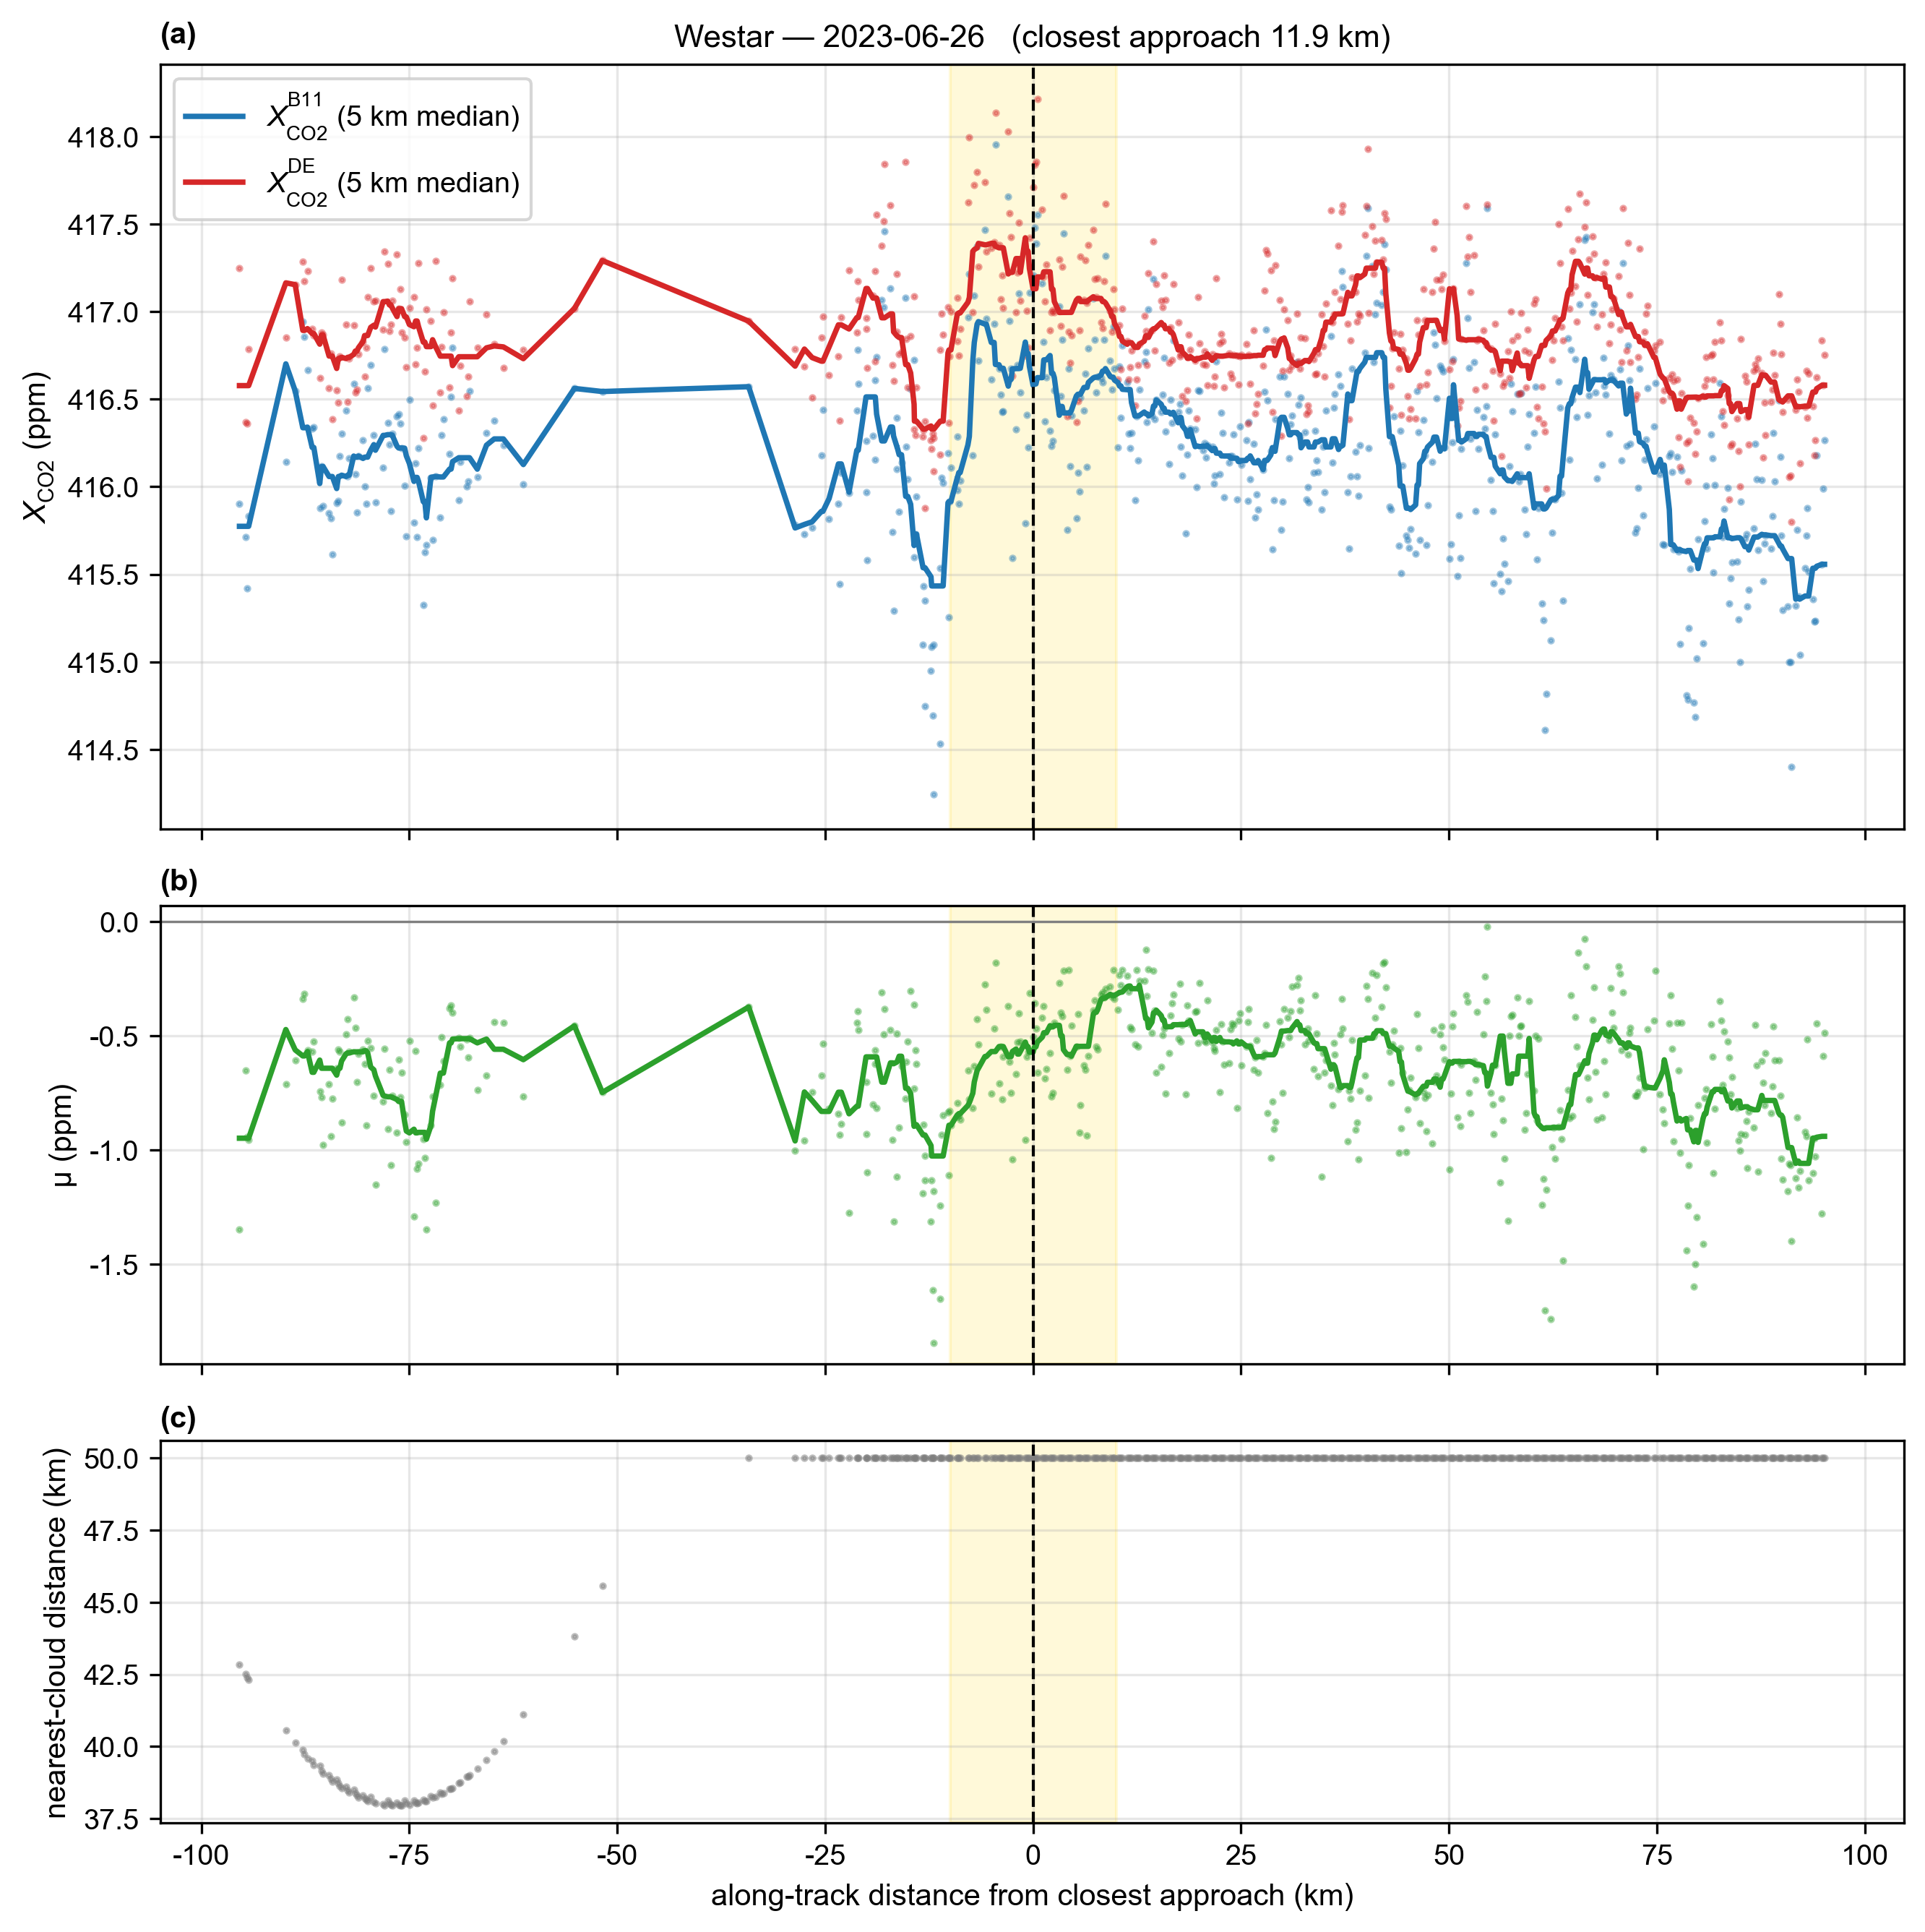
\includegraphics[width=0.65\textwidth]{figures/fig12a_westar_transect.png}\\[4pt]
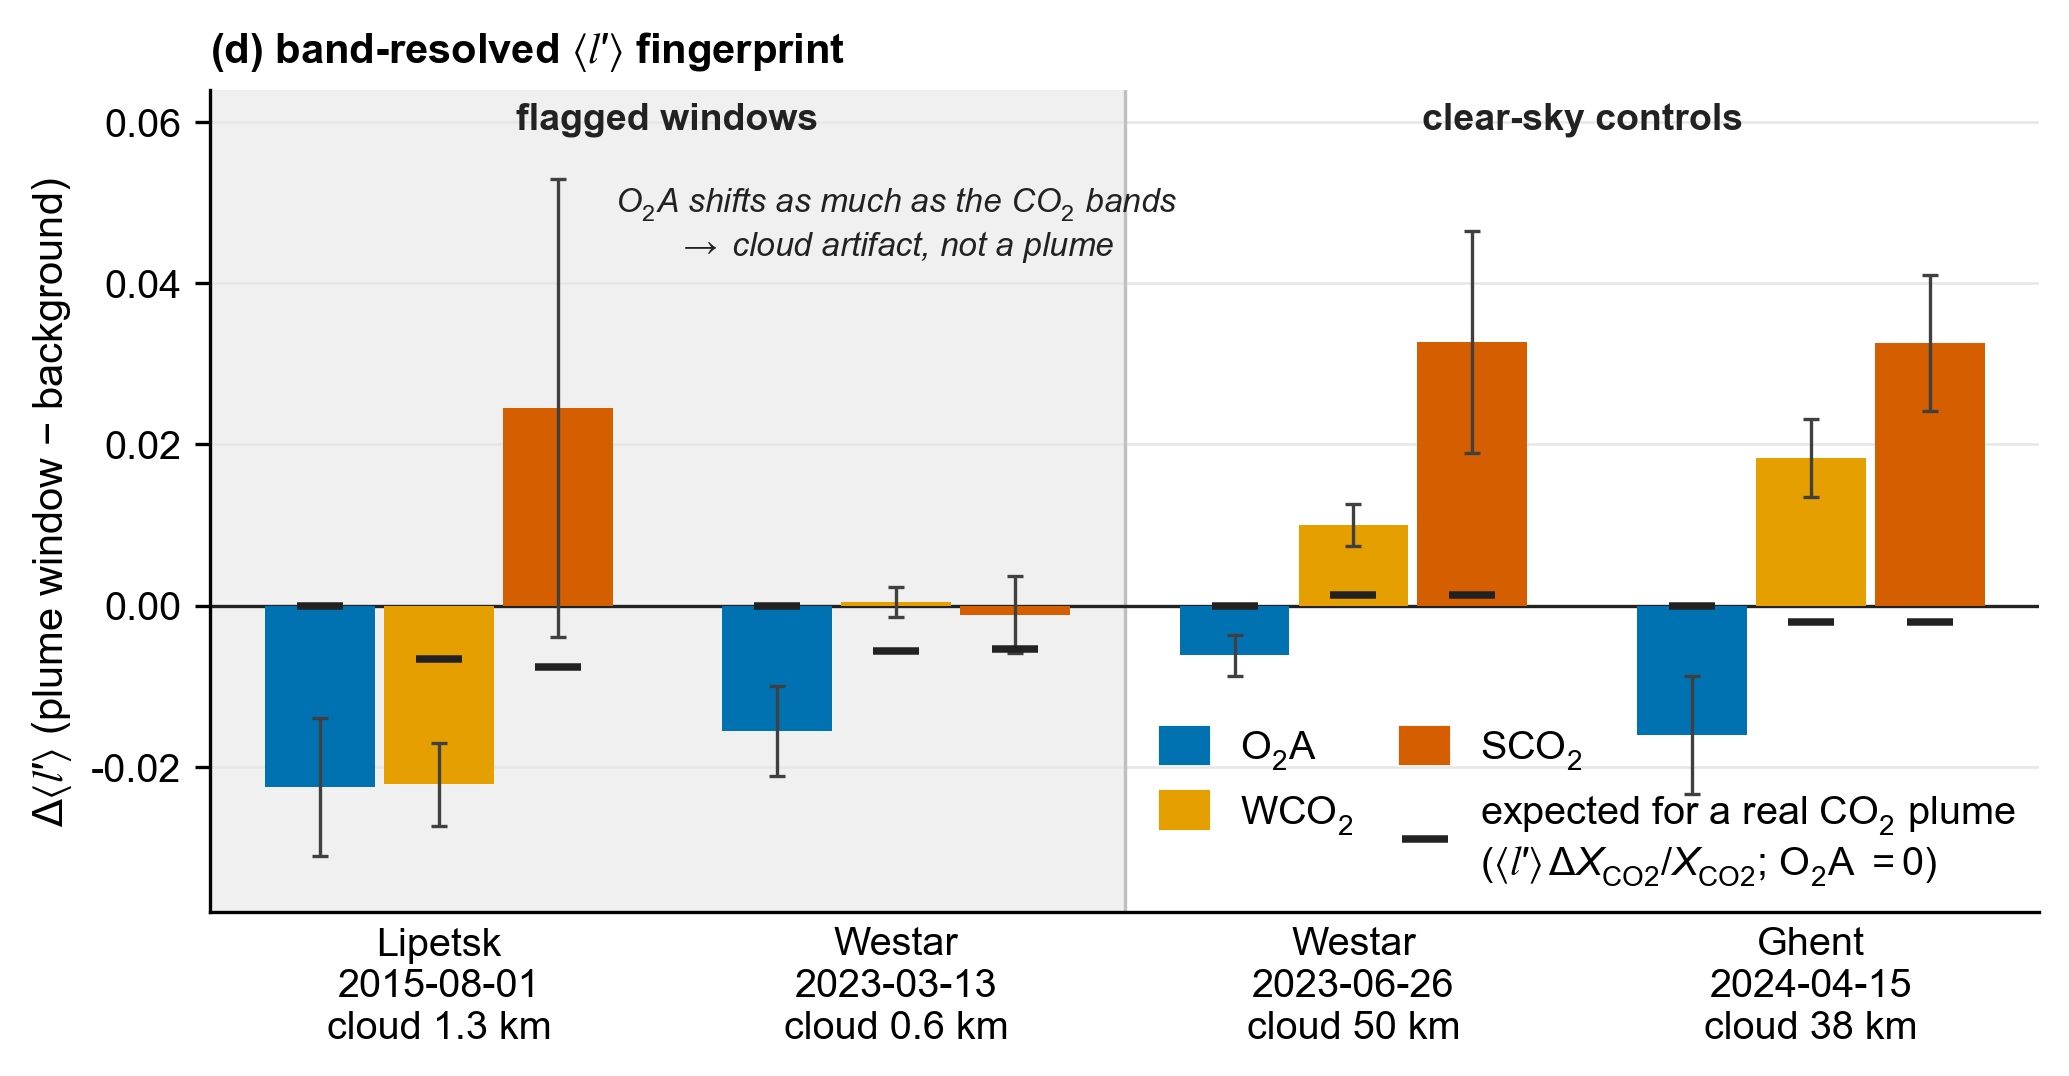
\includegraphics[width=0.65\textwidth]{figures/fig12b_k1_contrast.png}
\caption{Plume preservation and the spectral cloud fingerprint. (a) Along-track transect over the Westar power plant (26 June 2023, clear sky, nearest cloud ≈ 50 km; overpass from the Nassar et al. catalog) before and after correction; lower panels: predicted correction μ and nearest-cloud distance. (b) Band-resolved $\Delta$⟨$l'$⟩ (plume window minus background; ±1 SE) for the two flagged removal windows and two clear-sky controls. Black ticks: signature expected of a real CO2 plume ($\Delta$⟨$l'$⟩ ≈ ⟨$l'$⟩·$\Delta$\xco/\xco in the \ce{CO2} bands via the prior-based optical depth; exactly zero in \ce{O2}A).}
\label{fig:plume-preservation}
\end{figure}




\FloatBarrier